% PyBaMM Battery Modelling Conference 2026 — 1-page abstract, v7.
% Author: Krishna Chaitanya Vaddepally, Turno (Blubble Pvt. Ltd.)
% Deadline: 2026-07-15 UTC (max 1 A4 page, Arial >= 12 pt).
\documentclass[12pt,a4paper]{article}

\usepackage[T1]{fontenc}
\usepackage{amsmath,amssymb}
\usepackage{helvet}
\renewcommand{\familydefault}{\sfdefault}

\usepackage[a4paper,top=0.8cm,bottom=0.8cm,left=1.3cm,right=1.3cm]{geometry}
\usepackage{graphicx}
\usepackage{caption}
\captionsetup{font=footnotesize,labelfont=bf,labelsep=colon,skip=2pt}
\usepackage{microtype}
\usepackage[hidelinks]{hyperref}
\usepackage{enumitem}
\usepackage{float}

\pagestyle{empty}
\setlength{\parindent}{0pt}
\setlength{\parskip}{0.10em}

\begin{document}

\begin{center}
{\bfseries\large Cross-supplier SoH forecasting for second-life LFP cells\\
using a PyBaMM-trained neural operator}\\[0.35em]
\underline{Krishna Chaitanya Vaddepally}\\
\emph{Turno (Blubble Pvt.\ Ltd.), Bengaluru, India} \textbullet\
krishna.vaddepally@turno.club\\[0.15em]
{\footnotesize Theme: Data-driven Methods \textbullet\ Presentation: Oral (poster acceptable)}
\end{center}

Second-life reuse of retired lithium iron phosphate (LFP) cells is
limited by the cost of predicting future ageing for each cell.
Conventional lifetime testing takes months and empirical models often
transfer poorly across supplier-specific LFP cell designs. We present
a physics-conditioned neural operator that forecasts the future SoH
trajectory of a used LFP cell from a short diagnostic characterisation
plus the first 50 operating cycles, over an approximately 500-cycle
horizon into the deeper second-life regime.

\textbf{Workflow (Figure~\ref{fig:pipeline}).}
Seven anchor cells from three suppliers (CALB, EVE, REPT) are put
through a full R\&D characterisation suite ($\sim{}25$ days per anchor,
one-time cohort cost) and long-term-cycled at 0.25--0.5\,C.
Beginning-of-life and five degradation parameters (SEI growth,
lithium plating, negative-electrode active-material loss) are
identified by differential evolution against measured cycling. PyBaMM~[1]
SPMe on Prada2013 LFP chemistry~[2] then synthesises 490 perturbed
degradation trajectories around the anchors; SoH-offset augmentation
expands this to 14{,}096 (context,~target) training pairs covering the
second-life SoH range. A monotonic $\theta$-conditioned Neural ODE~[3]
with a learned context encoder combines three inference inputs: a
supplier-level $\theta$ prior from anchor DE fits, DCIR and
initial-capacity features from a $\sim{}2$-hour characterisation, and a
$K{=}50$-cycle SoH context window from the target cell.

\begin{figure}[H]
  \centering
  \IfFileExists{../V7_flowchart_cropped.png}{%
    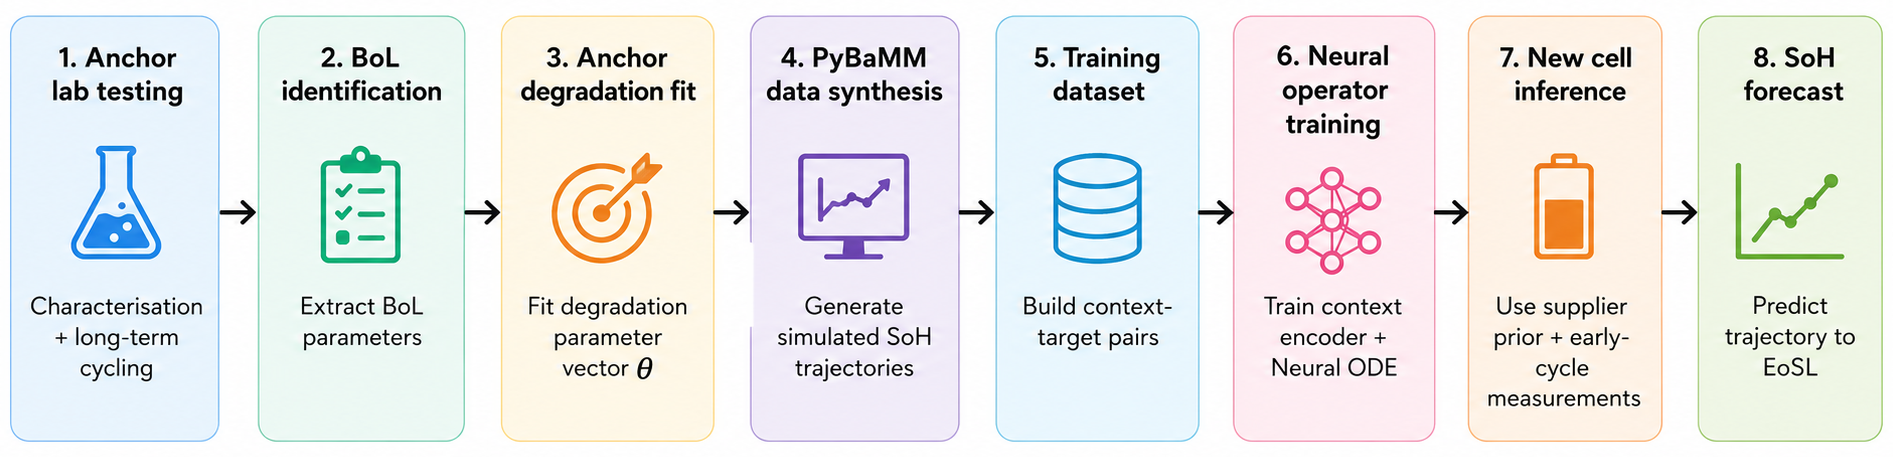
\includegraphics[width=0.68\textwidth]{../V7_flowchart_cropped.png}%
  }{%
    \fbox{\parbox[c][0.8cm][c]{0.9\textwidth}{\centering\footnotesize
      [placeholder: V7\_flowchart\_cropped.png]}}%
  }
  \caption{Pipeline: anchor characterisation and DE-fit feed a PyBaMM
  synthesis corpus; the SciML operator ingests $\theta$, DCIR/capacity
  features and $K{=}50$ observed cycles to forecast SoH.}
  \label{fig:pipeline}
\end{figure}

\textbf{Results.}
Evaluation on one cell per supplier that was excluded from
neural-operator training (CALB\_0029, EVE\_0003, REPT\_0028) gives SoH
RMSEs of 0.96, 0.79 and 0.47 percentage points on the experimentally
observed forecast region (Figure~\ref{fig:heldout}), mean 0.74~pp:
preliminary evidence of cross-supplier transfer within the evaluated LFP
families. The trained operator forecasts 500 cycles in \textbf{18\,ms}
($\sim{}350{\times}$ faster than the equivalent PyBaMM SPMe run). The
inference input (DCIR + RPT + 50 cycles at 0.5\,C) takes
$\sim{}12$ days per cell: \textbf{$\sim{}55\%$ shorter than the full
R\&D characterisation suite} and \textbf{$\sim{}55{\times}$ shorter than
cycle-to-EoL testing} ($\sim{}650$ days at the pilot anchor $\theta$).

\textbf{Limitations.} Cross-supplier claim rests on three excluded cells;
extrapolation beyond the observed cycling window is not yet
experimentally verified; baselines against linear/exponential fits and
the operator without SoH-offset augmentation are planned next.

\begin{figure}[H]
  \centering
  \IfFileExists{figures/heldout_v7_1_combined.pdf}{%
    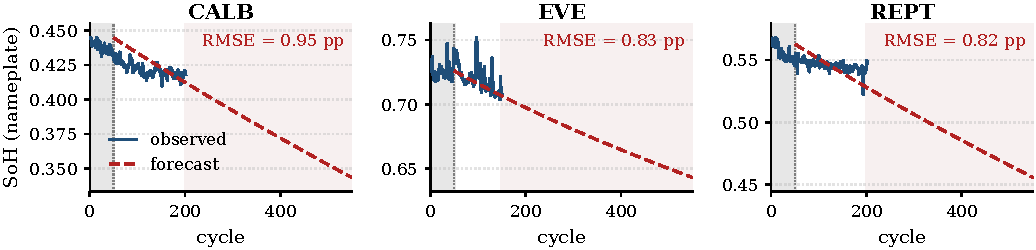
\includegraphics[width=0.74\textwidth]{figures/heldout_v7_1_combined.pdf}%
  }{%
    \fbox{\parbox[c][0.8cm][c]{0.9\textwidth}{\centering\footnotesize
      [placeholder: figures/heldout\_v7\_1\_combined.pdf]}}%
  }
  \caption{Held-out forecasts (one cell per supplier). Grey band =
  $K{=}50$ context; blue = observed; red dashed = forecast; pink band =
  unverified extrapolation beyond observed window. Per-cell RMSE 0.96,
  0.79, 0.47~pp (mean 0.74, std 0.20).}
  \label{fig:heldout}
\end{figure}

\vspace{-0.2em}
{\footnotesize
[1]~V.~Sulzer et al., \emph{J.\ Open Res.\ Software} \textbf{9} (2021), 14.
[2]~M.~Prada et al., \emph{J.\ Power Sources} \textbf{219} (2012), 353--362.
[3]~R.\,T.\,Q.~Chen et al., \emph{NeurIPS} (2018).
}

\end{document}
